\documentclass[11pt]{article}

\usepackage{amsmath}
\usepackage{amssymb}

\usepackage{graphicx}
\usepackage{tikz}

\usepackage{ytableau}

\usepackage{hyperref}

\title{Max-flow min-cut \\ Math 4707, Spring 2021}

\begin{document}


\maketitle

\thispagestyle{empty}


Find a maximum flow from from $s$ to $t$ in this network (where capacities are the edge labels):
\[ 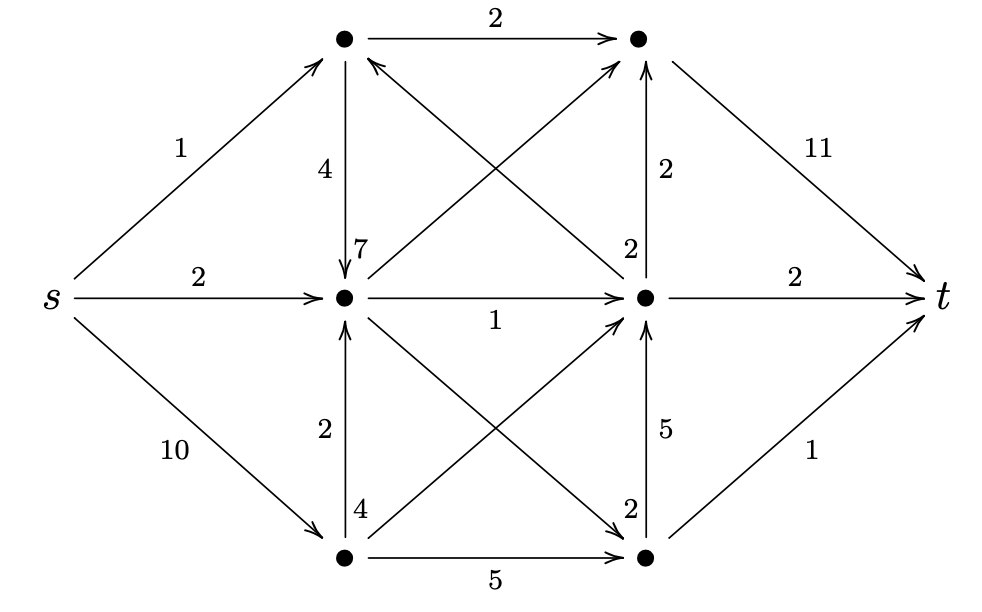
\includegraphics[width=4in]{network.png} \]
Hint: you can use the Ford-Fulkerson algorithm! In fact, you can go to this website: {\small \url{https://www-m9.ma.tum.de/graph-algorithms/flow-ford-fulkerson/index_en.html}} and use the applet there to input this graph and run the algorithm online.

Can you find a cut which proves your flow is a maximum flow?

\end{document}
